\documentclass[12pt]{article}

\usepackage[utf8]{inputenc}
\usepackage[russian]{babel}
\usepackage{amsmath, amssymb}
\usepackage{graphicx}
\usepackage{listings}

\lstset{
	language=Python,
	keepspaces=true,
	extendedchars=\true,
	inputencoding=utf8,
	basicstyle=\tiny,
	numbers=left,
	showspaces=false,
	showstringspaces=false,
}

\def\dd#1#2{\cfrac{\partial#1}{\partial#2}}
\def\ddd#1#2#3{\cfrac{\partial^2#1}{\partial#2\partial#3}}
\def\dddd#1#2{\cfrac{\partial^2#1}{\partial{#2}^2}}
\def \atxt#1{\left.#1\right|_{(\bar{x},\bar{t})}}

\author{Будакян Я. С.}

\begin{document}
	\begin{titlepage}
		\begin{center}
			{\small\textsc{Московский Государственный Университет им. М.\,В. Ломоносова}}
			\vskip 1pt \hrule \vskip 3pt
			{\small\textsc{Физический факультет}}
			\vfill
			{\Large Практическое задание по ОММ}
			\break
			\break
			{\Large Задача \#1}	
		\end{center}
		
		\vfill
		
		\begin{flushright}
			{Выполнил студент 335 группы\\Будакян Я.\,С.\\
			 Преподаватель Домбровская Ж.\,О.}
		\end{flushright}
	\end{titlepage}
	
	\section{Постановка задачи}
		\bigskip\par\noindent{\bf Задача 2. }
		Используя схему бегущего счета и итерационные методы, решить задачу:
		
		\begin{equation}\label{eq:problem}
			\begin{cases}
				&\dd{u}t - u\dd{u}x = 0, \quad -1 \le x < 0, \\
				&u(x, 0) = 2 - \frac{4}{\pi}\arctg(x+2), \\
				&u(0, t) = (2 - \frac{4}{\pi}\arctg2)e^{-t}
			\end{cases}
		\end{equation}
	
	\section{Метод решения}
		Во первых, чтобы определить, нет ли у решения разрыва, необходимо составить уравнение характеристик и посмотреть, пересекаются ли они:
		$$ \frac{dt}{1} = \frac{dx}{-u} = \frac{du}{0},$$
		откуда получаем:
		$$ du = 0 \rightarrow u = const,$$
		$$ dt = -\frac{1}{u}dx \rightarrow t - t_0 = -\frac{1}{u}(x - x_0)$$
		Подставив начальные условия, получаем уравнения для характеристик, выходящих из оси t:
		
		\begin{equation}\label{char_t0}
			x = (\frac{4}{\pi}\arctan2-2)(t-t_0)e^{-t_0},
		\end{equation}
		
		и оси x:
		
		\begin{equation}\label{char_x0}
			x = x_0 - t(2 - \frac{4}{\pi}\arctan(x_0+2))
		\end{equation}
		
		Построим графики семейств характеристик:
		\newpage
		
		\begin{figure}[h]
			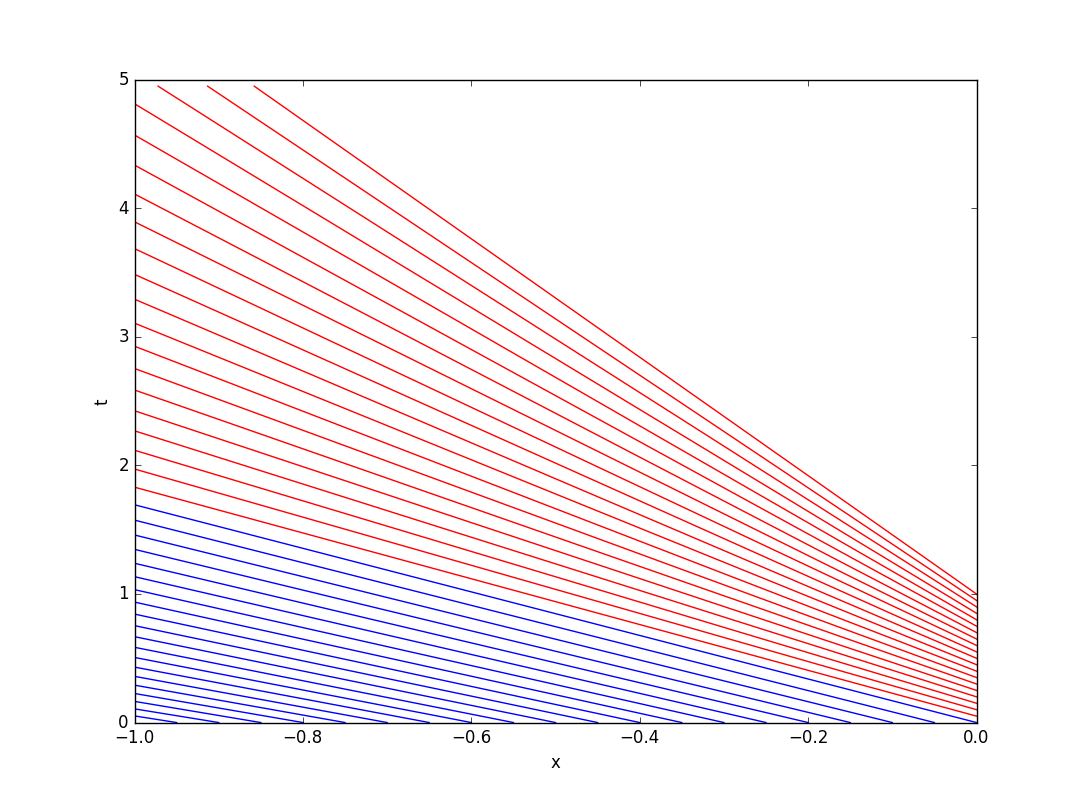
\includegraphics[scale = 0.5]{char_1}
			\caption{Семейства характеристик, красные соответствуют (\ref{char_t0}), синие - (\ref{char_x0})}
		\end{figure}
		
		Как видно из рисунка, в рассматриваемой области $ -1 \leq x < 0 $ характеристики не пересекаются. Следовательно, временной интервал расчета может быть выбран произвольно, например, $t \in [0, 1]$.
		Введем равномерные разностные сетки:
		
		$$\bar{\omega}_h = \{x_i = ih;\ i = \overline{0,N};\ hN = 1\}$$
		$$\bar{\omega}_\tau = \{t_j = j\tau;\ j =\overline{0,S};\ \tau S = T\}$$
		$$\bar{\omega}_{h\tau} = \bar{\omega}_h \times \bar{\omega}_\tau = 
		\{ (x_i, t_j) \in \bar{D} \}$$
		$$\bar{D} = \{ -1 \le x < 0;\ 0 \le t \le T \}$$
		
		Перепишем основное уравнение (\ref{eq:problem}) в дивергентном виде:
		
		\begin{equation}
			\dd{u}t + \dd{}x\left(\frac{-u^2}{2}\right) = 0
		\end{equation}
		
		Введем сеточную функцию:
		
		$$y_i^j \overset{\mathrm{def}}{=} u(x_i, t_j)$$
		
		Запишем разностную схему задачи (\ref{eq:problem}), используя неявный четырехточечный шаблон с весовыми пространственными и временными производными с весом $\sigma = \frac{1}{2}$ :
		
		\begin{figure}[h!]
			\begin{center}
				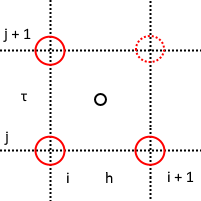
\includegraphics[width=0.5\linewidth]{template}
				\caption{Шаблон "прямоугольник"\,, i - x, j - t}
			\end{center}
		\end{figure}
		
		\begin{equation}
			\frac{y^{j+1}_i - y^j_i + y^{j+1}_{i+1} - y^j_{i+1}}{2\tau} + \frac{F^j_{i+1} - F^j_i + F^{j+1}_{i+1} - F^{j+1}_i}{2h} = 0,
		\end{equation}
		
		где $F^j_i \overset{\mathrm{def}}{=} -\frac{(y^j_i)^2}{2}$. Запуская схему бегущего счета с известных граничных и начальных значений, можно последовательно определить всю сеточную функцию. Для вычисления новой точки $y^{j+1}_{i+1}$ нужно решить возникающее алгебраическое уравнение, например, итерационным методом. Определим функцию:
		
		$$ f(x) \overset{\mathrm{def}}{=} \frac{y^{j+1}_i - y^j_i + x - y^j_{i+1}}{2\tau} + \frac{F^j_{i+1} - F^j_i + F(x) - F^{j+1}_i}{2h}$$
		Для корня $f(x) = 0$ справедливо
		$$x_{n+1} = x_n - \frac{f(x_n)}{f'(x_n)}$$
		
		В качестве начального приближения можно взять $x_0 = y_i^{j+1}$.\\
		Определим порядок аппроксимации построенной разностной схемы. Для этого введем функцию погрешности
		
		\begin{equation}
			\psi_{h\tau} = \frac{y^{j+1}_i - y^j_i + y^{j+1}_{i+1} - y^j_{i+1}}{2\tau} + \frac{F^j_{i+1} - F^j_i + F^{j+1}_{i+1} - F^{j+1}_i}{2h} - \dd{u}t - \dd{F}u\dd{u}x
		\end{equation}
		
		и разложим ее в ряд Тейлора в центральной точке шаблона
		
		$$(\bar{x}, \bar{t}) = (x_i + \frac{h}{2}, t_j + \frac{\tau}{2}):$$
		
		\begin{multline}
			y^{j+1}_{i+1} = y(\bar{x} + \frac{h}{2}, \bar{t} + \frac{\tau}{2}) =  y(\bar{x}, \bar{t}) + \frac{h}{2}\atxt{\dd{u}t} + \frac{\tau}{2}\atxt{\dd{u}x} +\\
			+ \frac{1}{2}\atxt{\left\{ \frac{h^2}{4}\dddd{u}x + \frac{\tau^2}{4}\dddd{u}t + \frac{h\tau}{4}\ddd{u}{x}t \right\}} + o(h^3 + \tau^3)
		\end{multline}
		
		\begin{multline}
			y^{j}_{i+1} = y(\bar{x} + \frac{h}{2}, \bar{t} - \frac{\tau}{2}) =  y(\bar{x}, \bar{t}) + \frac{h}{2}\atxt{\dd{u}t} - \frac{\tau}{2}\atxt{\dd{u}x} +\\
			+ \frac{1}{2}\atxt{\left\{ \frac{h^2}{4}\dddd{u}x + \frac{\tau^2}{4}\dddd{u}t - \frac{h\tau}{4}\ddd{u}{x}t \right\}} + o(h^3 + \tau^3)
		\end{multline}
		
		\begin{multline}
			y^{j+1}_{i} = y(\bar{x} - \frac{h}{2}, \bar{t} + \frac{\tau}{2}) =  y(\bar{x}, \bar{t}) - \frac{h}{2}\atxt{\dd{u}t} + \frac{\tau}{2}\atxt{\dd{u}x} +\\
			+ \frac{1}{2}\atxt{\left\{ \frac{h^2}{4}\dddd{u}x + \frac{\tau^2}{4}\dddd{u}t - \frac{h\tau}{4}\ddd{u}{x}t \right\}} + o(h^3 + \tau^3)
		\end{multline}
		
		\begin{multline}
			y^{j}_{i} = y(\bar{x} - \frac{h}{2}, \bar{t} - \frac{\tau}{2}) =  y(\bar{x}, \bar{t}) - \frac{h}{2}\atxt{\dd{u}t} - \frac{\tau}{2}\atxt{\dd{u}x} +\\
			+ \frac{1}{2}\atxt{\left\{ \frac{h^2}{4}\dddd{u}x + \frac{\tau^2}{4}\dddd{u}t + \frac{h\tau}{4}\ddd{u}{x}t \right\}} + o(h^3 + \tau^3)
		\end{multline}

		\begin{multline}
			F^{j+1}_{i+1} = F(y^{j+1}_{i+1}) = F(y(\bar{x} + \frac{h}{2}, \bar{t} + \frac{\tau}{2})) =  F(y(\bar{x}, \bar{t})) + \frac{h}{2}\dd{F}u\atxt{\dd{u}x} + \\
			+\frac{\tau}{2}\dd{F}u\atxt{\dd{u}t} + \frac{1}{2}\atxt{\left\{ \frac{h^2}{4}\left[ \dddd{F}u \left( \dd{u}x\right)^2 + \dddd{u}x\dd{F}u \right] + \frac{\tau^2}{4}\left[ \dddd{F}u\left( \dd{u}t \right)^2 + \dddd{u}t\dd{F}u \right] \right\}}+\\
			+ \frac{1}{2}\atxt{\left\{ \frac{h\tau}{4}\left[ \dddd{F}u\dd{u}x\dd{u}t + \ddd{u}{x}t\dd{F}u \right] \right\}} + o(h^3 + \tau^3)
		\end{multline}
		
		\begin{multline}
			F^{j}_{i+1} = F(y^{j}_{i+1}) = F(y(\bar{x} + \frac{h}{2}, \bar{t} - \frac{\tau}{2})) =  F(y(\bar{x}, \bar{t})) + \frac{h}{2}\dd{F}u\atxt{\dd{u}x} - \\
			-\frac{\tau}{2}\dd{F}u\atxt{\dd{u}t} + \frac{1}{2}\atxt{\left\{ \frac{h^2}{4}\left[ \dddd{F}u \left( \dd{u}x\right)^2 + \dddd{u}x\dd{F}u \right] + \frac{\tau^2}{4}\left[ \dddd{F}u\left( \dd{u}t \right)^2 + \dddd{u}t\dd{F}u \right] \right\}}+\\
			+ \frac{1}{2}\atxt{\left\{ -\frac{h\tau}{4}\left[ \dddd{F}u\dd{u}x\dd{u}t + \ddd{u}{x}t\dd{F}u \right] \right\}} + o(h^3 + \tau^3)
		\end{multline}

		\begin{multline}
			F^{j+1}_{i} = F(y^{j+1}_{i}) = F(y(\bar{x} - \frac{h}{2}, \bar{t} + \frac{\tau}{2})) =  F(y(\bar{x}, \bar{t})) - \frac{h}{2}\dd{F}u\atxt{\dd{u}x} + \\
			+\frac{\tau}{2}\dd{F}u\atxt{\dd{u}t} + \frac{1}{2}\atxt{\left\{ \frac{h^2}{4}\left[ \dddd{F}u \left( \dd{u}x\right)^2 + \dddd{u}x\dd{F}u \right] + \frac{\tau^2}{4}\left[ \dddd{F}u\left( \dd{u}t \right)^2 + \dddd{u}t\dd{F}u \right] \right\}}+\\
			+ \frac{1}{2}\atxt{\left\{ -\frac{h\tau}{4}\left[ \dddd{F}u\dd{u}x\dd{u}t + \ddd{u}{x}t\dd{F}u \right] \right\}} + o(h^3 + \tau^3)
		\end{multline}
		
		\begin{multline}
			F^{j}_{i} = F(y^{j}_{i}) = F(y(\bar{x} - \frac{h}{2}, \bar{t} - \frac{\tau}{2})) =  F(y(\bar{x}, \bar{t})) - \frac{h}{2}\dd{F}u\atxt{\dd{u}x} - \\
			-\frac{\tau}{2}\dd{F}u\atxt{\dd{u}t} + \frac{1}{2}\atxt{\left\{ \frac{h^2}{4}\left[ \dddd{F}u \left( \dd{u}x\right)^2 + \dddd{u}x\dd{F}u \right] + \frac{\tau^2}{4}\left[ \dddd{F}u\left( \dd{u}t \right)^2 + \dddd{u}t\dd{F}u \right] \right\}}+\\
			+ \frac{1}{2}\atxt{\left\{ \frac{h\tau}{4}\left[ \dddd{F}u\dd{u}x\dd{u}t + \ddd{u}{x}t\dd{F}u \right] \right\}} + o(h^3 + \tau^3)
		\end{multline}
		
		После подстановки и приведения подобных, получаем
		
		$$\psi_{h\tau} = o(h^2+\tau^2)$$
		
		Для того, чтобы выбрать шаг сетки по времени и координатам, необходимо проверить устойчивость разностной схемы. Это можно сделать с помощью метода замороженных коэффициентов и спектрального критерия Неймана(в задачах переноса, критерий Неймана является не только необходимым, но и достаточным условием устойчивости). Для этого будем рассматривать линейное уравнение $\dd{u}t + c\dd{u}x$, где $c = -u(x^*,t^*)$ - "замороженный коэффициент" в некоторой точке $(x^*,t^*)$. Утверждается, что если схема безусловно устойчива, то она будет устойчива и при условиях вида $y^m_n = \lambda^m e^{i\alpha n}$. Подставим в разностную схему:
		
		\begin{equation}
			\frac{1}{2\tau}\left\{ y^{m+1}_n - y^m_n + y^{m+1}_{n+1} - y^m_{n+1} \right\} + \frac{c}{2h}\left\{ y^m_{n+1} - y^m_n + y^{m+1}_{n+1} - y^{m+1}_n \right\} = 0
		\end{equation}
		
		\begin{multline}
			\frac{1}{\tau}\left\{ \lambda^{m+1}e^{i\alpha n} - \lambda^m e^{i\alpha n} + \lambda^{m+1}e^{i\alpha(n+1)} - \lambda^m e^{i\alpha(n+1)} \right\} +\\
			+ \frac{c}{h}\left\{ \lambda^m e^{i\alpha(n+1)} - \lambda^m e^{i\alpha n} + \lambda^{m+1}e^{i\alpha(n+1)} - \lambda^{m+1}e^{i\alpha n} \right\} = 0
		\end{multline}
		
		\begin{equation}
			\frac{1}{\tau}\left\{ \lambda - 1 + \lambda e^{i\alpha} - e^{i\alpha} \right\} + \frac{c}{h}\left\{ e^{i\alpha} - 1 + \lambda e^{i\alpha} - \lambda \right\} = 0
		\end{equation}
		
		\begin{equation}
			\lambda = \frac{h(1+e^{i\alpha} + c\tau(1-e^{i\alpha}))}{h(1+e^{i\alpha} + c\tau(e^{i\alpha}-1))} = \frac{ictg(\frac{\alpha}{2}) + r}{ictg(\frac{\alpha}{2})-r},
		\end{equation}
		
		где $r = \frac{c\tau}{h}$. Получаем, что $|\lambda| = 1$, что означает выполнение спектрального критерия. Следовательно, выбор параметров $h$ и $\tau$ может быть произволен.
		
		\newpage
		\section{Результаты}
		Численный расчет с помощью описанного алгоритма дает следующий результат:
		
		\begin{figure}[h!]
			\begin{minipage}[h]{0.73\linewidth}
				\center{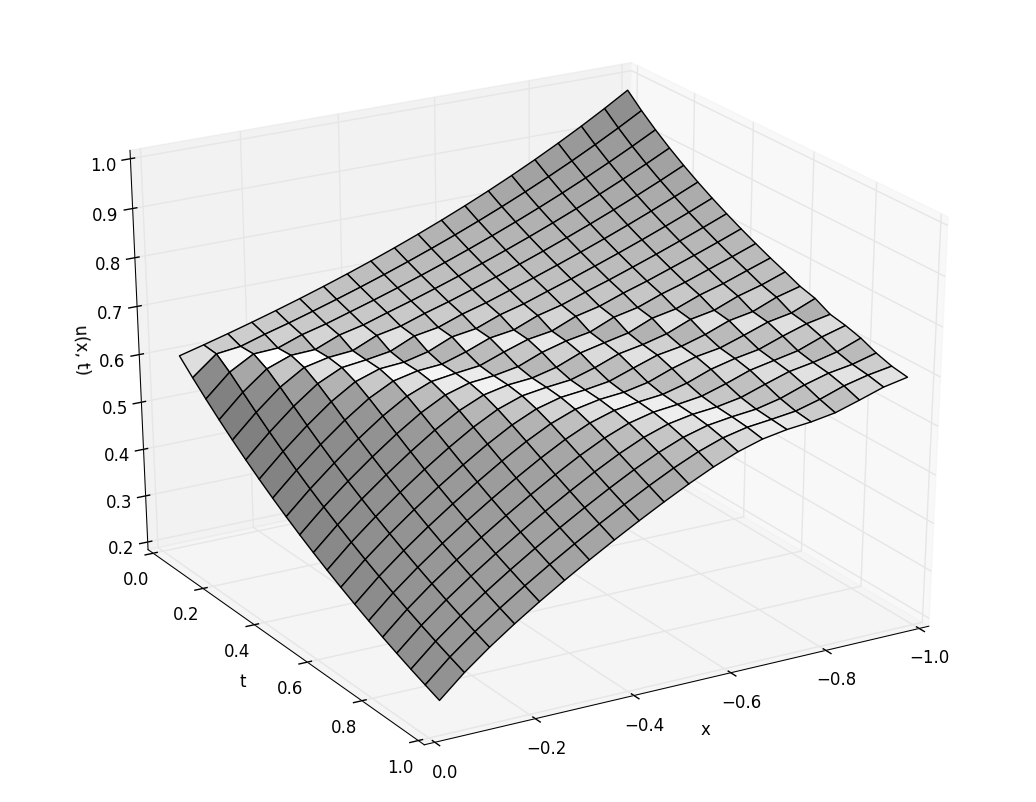
\includegraphics[width=1\linewidth]{solution_1}}
			\end{minipage}
			
			\begin{minipage}[h]{0.73\linewidth}
				\center{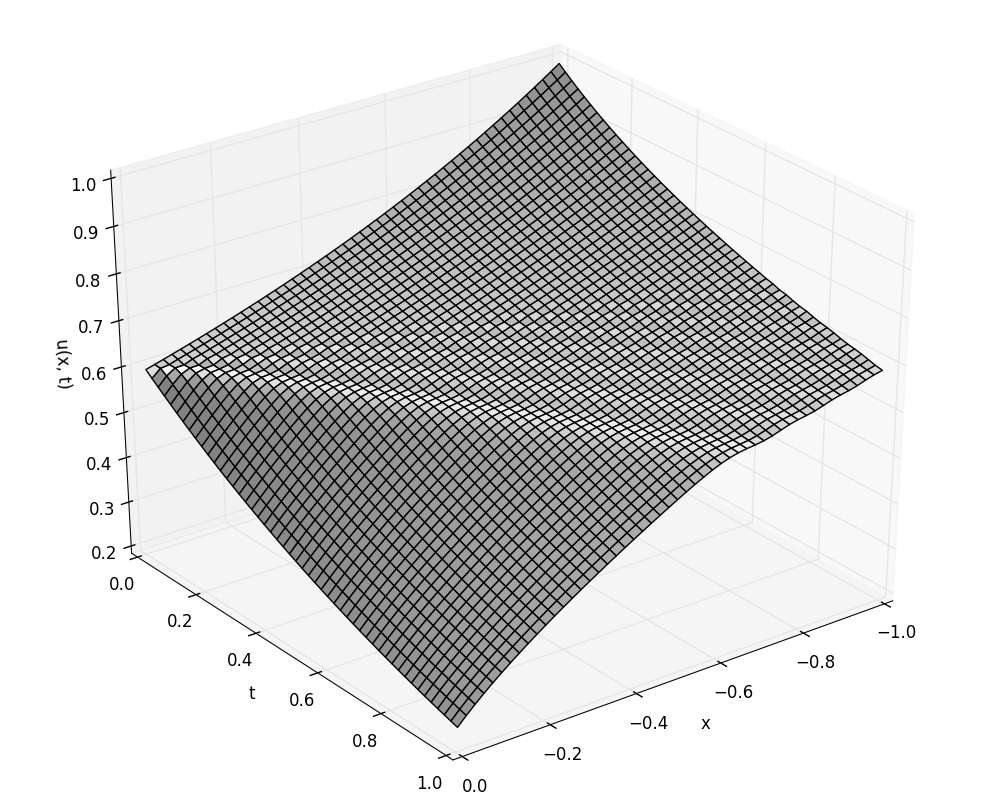
\includegraphics[width=1\linewidth]{solution_2}}
			\end{minipage}
		\end{figure}
		
		\newpage
		\section{Листинг программы}
		\lstinputlisting{solution.py}
		
\end{document}
